\documentclass{standalone}
\usepackage{tikz}
\usepackage{graphicx}
\usetikzlibrary{arrows.meta, decorations.pathmorphing, positioning}

\usepackage{float}

\begin{document}

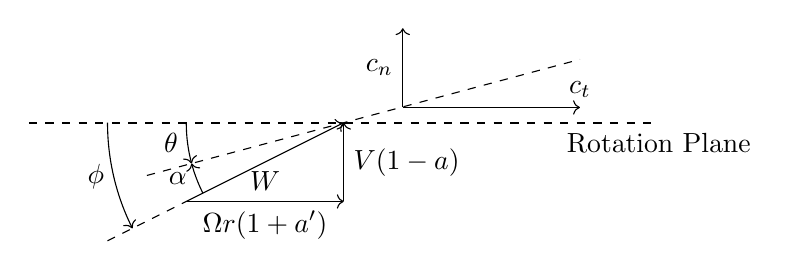
\begin{tikzpicture}
        % Some profiles look better when using plot[smooth]
    \begin{scope}[rotate=15]
        \draw[scale=3,thick=3] node[left=0.5cm] {}
            plot file{../../../app/foils/NACA2412.surf} -- cycle;
    \end{scope}
    % hoirzontal line
    \draw[thick, dashed] (-4,0) -- (4, 0) node[below] {Rotation Plane};
    % velocity vector labelled at midline
    \draw[->] (0,-1) -- (0,0) node[midway,right] {$V(1-a)$};
    \draw[->] (-2,-1) -- (0,-1) node[midway,below] {$\Omega r(1+a')$};
    \draw[->] (-2,-1) -- (0,0) node[midway,below] {$W$};
    \draw[dashed] (-3,-1.5) -- (-2,-1) node[above] {};
    \draw[dashed] (-2.5,-0.67) -- (3,0.804) node[above] {};
    % curved arrows
    \draw[->] (-2,0) arc (0:15:-2) node[midway, left] {$\theta$};
    \draw[->] (-3,0) arc (0:26.565:-3) node[midway, left] {$\phi$};
    \draw[->] (-1.7888,-0.8944) arc (26.565:15:-2) node[midway, left] {$\alpha$};
    % force coefficients
    \draw[->] (0.75, 0.194) -- (0.75,1.2) node[midway, left] {$c_n$};
    \draw[->] (0.75, 0.194) -- (3, 0.194) node[above] {$c_t$};
\end{tikzpicture}

\end{document}